\documentclass{cmc}
\usepackage{makecell}
\usepackage{enumitem}
% \usepackage{subfig}
\begin{document}

\pagestyle{fancy}
\lhead{\textit{\textbf{Computational Motor Control, Spring 2023} \\
    Final project, Project 1, GRADED}} \rhead{Student \\ Names}

\section*{Student names: \ldots (please update)}

\textit{
  Please note that
  this project is \textbf{\corr{graded}}. \textbf{\corr{The project will be graded in two parts}}.
  Part 1(Project 1) is about implementing an open-loop bio-inspired controller for an
  amphibious robot. Part 2( Project 2)  dives into sensory feedback and how to incorporate
  it for our controler. Project 1 has 5 exercise (p1 to p5) and project 2 has one exercise p6.
  Project 2 will is scheduled to be released on Friday 14/05/2023.
}

\textit{
  \textbf{\corr{Deadlines: Project 1: Friday 19/05/2023 23:59 Project 2: Friday 02/06/2023 23:59}}
}

\textbf{Instructions}

\begin{itemize}
  \item \textit{
    Update this file (or recreate a similar one, e.g.\ in
    Word) to prepare your answers to the questions. Feel free to add text,
    equations and figures as needed. Hand-written notes, e.g.\ for the development
    of equations, can also be included e.g.\ as pictures (from your cell phone or
    from a scanner).
  }
  \item \textit{Submit project 1 and project 2 \corr{reports} separately.}
  \begin{itemize}
    \item \textit{project 1 should contain exercise 1 to 5.}
    \item \textit{project 2 should contain exercise 6.}
  \end{itemize}
  \item \textit{ Please submit both the source file.
    (*.doc/*.tex) and a pdf of your document, as well as all the used and updated
    python code can be submitted in a single zipped file called \newline
    \corr{final\_report\_name1\_name2\_name3.zip} where name\# are the team
    member's last names.  \corr{Please submit only one report per team!}
  }
\end{itemize}

%%%%%%%%%%%%%%%%%%%%%%%%%%%%%%%%%%%%%%%%%%%%%%%%%%%%%%%%%%%%%%%%%%%%%%%%%%%%%%%%%%%%%%%%%%%%%%%%%%%%
% \section*{Questions}
\section*{Amphibious Locomotion with Polymander --- CPG Model}\label{sec:exploring-swimming}

In this project you will control a salamander-like robot poymander
 for which you will use Python and the MuJoCo physics
engine. You have an opportunity to use what you've learned until
now to make the robot swim and walk in open and closed loop scenarios.
In order to do this, you should implement a CPG based swimming controller,
similarly to the architecture shown in Figure~\ref{fig:controller-model-spine} and~\ref{fig:controller-model-leg}.

The project is based on the research of~\cite{Crespi2013},
~\cite{Karakasiliotis2013},~\cite{ijspeert2007swimming}
and~\cite{thandiackal2021emergence}. It is strongly recommended to
review~\cite{ijspeert2007swimming},~\cite{owaki2013simple} and their
supplementary material provided on the Moodle.
You will be tasked with replicating and studying the
Central Pattern Generator (CPG) network proposed in those papers.

\begin{figure}[H]
  \centering
  \includegraphics[width=0.8\textwidth]{figures/Polymander_controller_spine.png}
  \caption[Controller model spine]{A double chain of oscillators controlling
    the robot's spine.}\label{fig:controller-model-spine}
\end{figure}

\begin{figure}[H]
  \centering
  \includegraphics[width=0.8\textwidth]{figures/Polymander_controller_leg.png}
  \caption[Controller model limbs]{Single oscillators for each limb}
  \label{fig:controller-model-leg}
\end{figure}



% \newpage

\subsection*{Code organization}\label{subsec:code}

\begin{figure}[ht]
  \centering 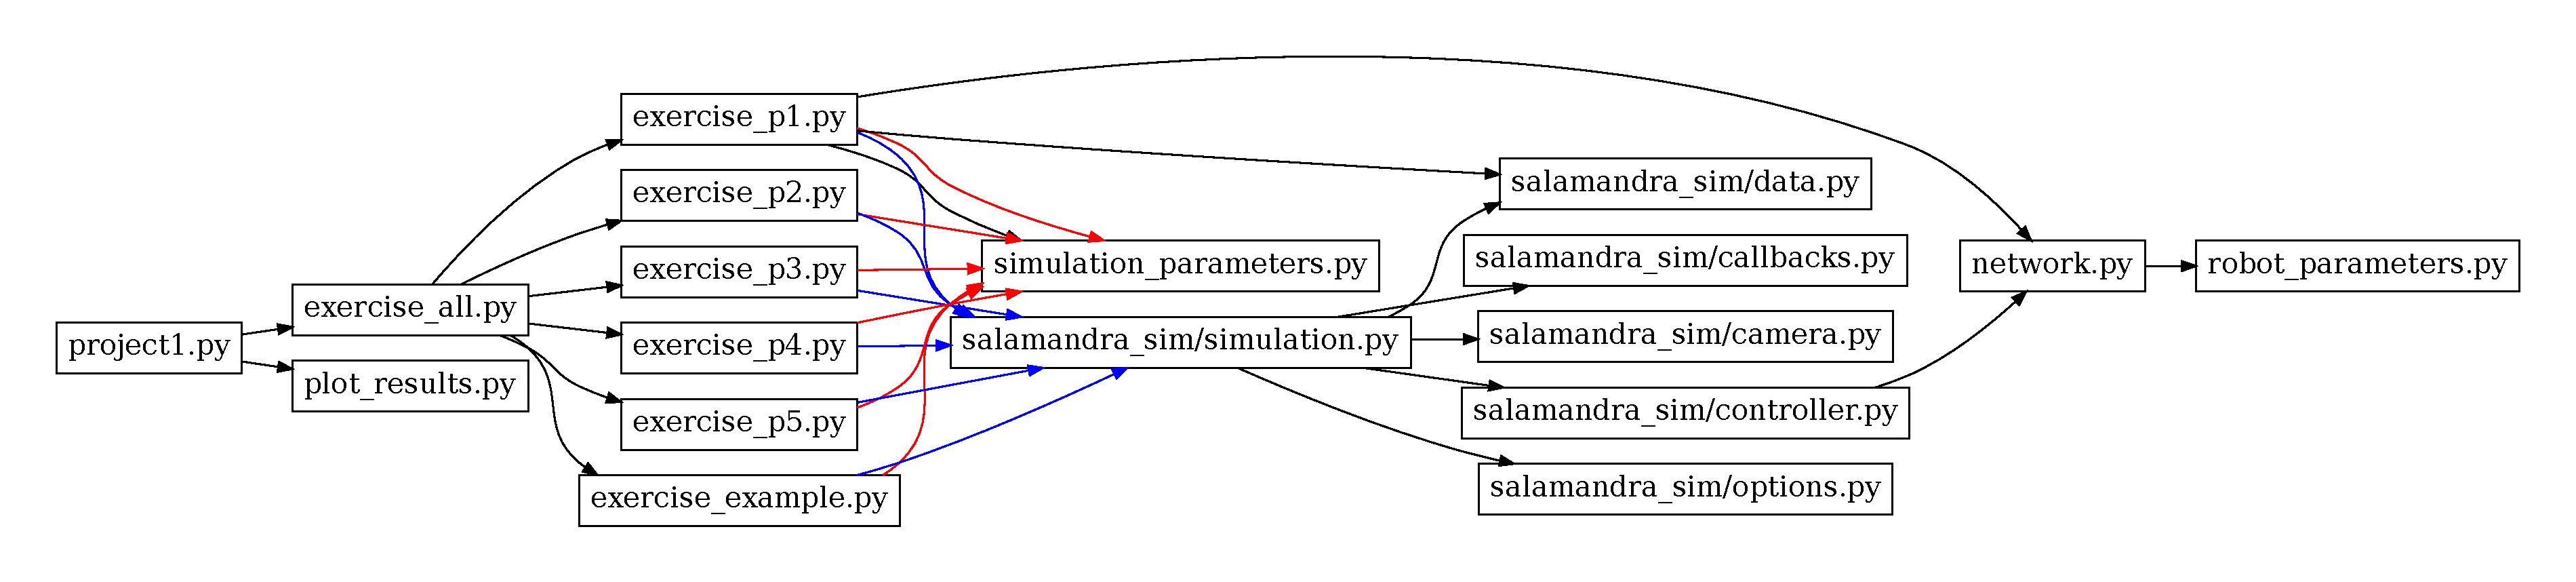
\includegraphics[width=1.0\textwidth]{figures/files}
  \caption{\label{fig:files} Exercise files dependencies. In this lab, you will
    be modifying \fileref{exercise\_\#.py}, \fileref{network.py},
    \fileref{robot\_parameters.py} and \fileref{simulation\_parameters.py}}
\end{figure}

\begin{itemize}
\item \corr{\textbf{project1.py}} --- A convenient file for running the entire
  project. Note you can also run the different exercises in parallel by
  activating \texttt{parallel=True}. \textit{You do not need to modify this
    file.}
\item \corr{\textbf{exercise\_all.py}} --- Another convenient file for running all
  or specified exercises depending on arguments provided. \textit{You do not
    need to modify this file.}
\item \corr{\textbf{network.py}} --- This file contains the different classes and
  functions for the CPG network and the Ordinary Differential Equations
  (ODEs). You can implement the network parameters and the ODEs here. Note that
  some parameters can be obtained from robot\_parameters.py to help you control
  the values.
\item \corr{\textbf{robot\_parameters.py}} --- This file contains the different
  classes and functions for the parameters of the robot, including the CPG
  network parameters. You can implement the network parameters here. Note that
  some parameters can be obtained from the SimulationParameters class in
  \corr{simulation\_parameters.py} and provided in \corr{exercise\_\#.py} to
  help you control the values (refer to example.py).
\item \corr{\textbf{simulation\_parameters.py}} --- This file contains the
  SimulationParameters class and is provided for convenience to send parameters
  to the setup of the network in \corr{network.py::SalamandraNetwork} via the
  robot parameters in \corr{robot\_parameters.py::RobotParameters}. The
  SimulationParameters is also intended to be used for experiment-specific
  parameters for the exercises. All the values provided in SimulationParameters
  are logged for each simulation, so you can also reload these parameters when
  analyzing the results of an experiment.
\item \corr{\textbf{exercise\_p1.py}} --- By running the script from Python,
  MuJoCo will be bypassed and you will run the network without a physics
  simulation. Make sure to use this file for question 1 to help you with
  setting up the CPG network equations and parameters and to analyze its
  behavior. This is useful for debugging purposes and rapid controller
  development since running the MuJoCo simulation takes more time.
\item \corr{\textbf{exercise\_example.py}} --- Contains the example code structure
  to help you familiarize with the other exercises. \textit{You do not need to
    modify this file.}
\item \corr{\textbf{exercise\_\#.py}} --- To be used to implement and answer the
  respective exercise questions. Note that \corr{exercise\_example.py} is
  provided as an example to show how to run a parameter sweep. Note that network
  parameters can be provided here.
\item \corr{\textbf{exercise\_all.py}} --- A convenient file for running different
  exercises depending on arguments. See \corr{\textbf{project1.py}} for an example
  on how to call it. \textit{You do not need to modify this file.}
\item \corr{\textbf{plot\_results.py}} --- Use this file to load and plot the
  results from the simulation. This code runs with the original example provided
  and provides examples on how to collect the data. It also contains the implementation
  for the performance metrics described below.
\item \corr{\textbf{salamandra\_simulation folder}} --- Contains all the remaining
  scripts for setting up and running the simulation experiments. \textit{You do
    not need to modify any of these file but should still go through them to get
    a better understanding of the code.}
\end{itemize}

% \newpage

\section*{Prerequisites}
To have all the necessary python packages necessary to complete the
final project, check that you have installed all the necessary required packages.
Next, pull the latest version of the exercise repository. Navigate to the
location of your repository in the terminal and execute the following,

\begin{lstlisting}[language=Bash]
  >> pip install -r requirements.txt
\end{lstlisting}


\subsection*{Simulation environment installation}

The installation of the simulation environment can be completed using a script
found in the Python folder of Project 1. You can run it by simply calling:

\label{sec:mujoco-inst}
\begin{lstlisting}[language=Bash]
  >> python setup_sim_env.py
\end{lstlisting}

This will install the \textit{MuJoCo} simulator and the \textit{dm\_control}
package which are software maintained by Deepmind for running robot
simulations. It will also install the \textit{farms\_core},
\textit{farms\_mujoco} and \textit{farms\_sim} packages developed at the
Biorobotics Laboratory (BioRob). If you are interested in knowing more about
\textit{MuJoCo}, you can find out more on \href{https://mujoco.org/}{\corr{the
    official website}}.

\corr{\textit{IMPORTANT:}} Make sure you have activated and are using your
virtual environment and its python interpreter that that you have created for
this course.

\corr{\textit{NOTE:}} If you are unclear about the basic steps then refer back
to Lab 0 documentation here
\href{https://farmsim.gitlab.io/courses/cmc-2023/}{\corr{cmc-installation-help}}


\subsection*{Examples}
You can run a simulation example to get you accustomed
to the MuJoCo graphical interface with \corr{\textbf{exercise\_example.py}}. You
should see the polymander model floating on the water. Try running:
\label{sec:mujoco-example}
\begin{lstlisting}[language=Bash]
  >> python exercise_example.py
\end{lstlisting}

\subsubsection*{Graphical User Interface Interaction}
When you run the example script, a Graphical User Interface (GUI) should launch.
You can use the left mouse click to move around the scene and right mouse click
to rotate the camera. You can also select a part of the robot by double left
clicking on a part. Once selected, you can then interact with it by holding the
CONTROL key and dragging with left or right click. Try it out for yourself to
familiarise with the interface.

There are many keyboard shortcuts also available

\begin{itemize}
\item Press SPACE to toggle play/pause
\item Press ``\textquotesingle'' / ``\textsuperscript{$\wedge$}'' to change
  speed factor (between zero (0) and backspace)
\item Press w to toggle wireframe
\item Press t to toggle transparency
\item Press s to toggle shadows
\item Press c to show collisions
\item Press f to show collisions forces, combine with p to show
  friction/reaction
\item Press b to show external forces (try in water later on)
\item And many more...
\end{itemize}

\textbf{Important things to explore with the provided example}
\begin{itemize}
\item Changing the view of the scene using the controls above
\item Interaction with the objects in the scene
\item Try changing to a water arena in the example script and showing the forces
  acting on the body (b)
\end{itemize}

\subsection*{Preparing for the project}
Once you are done with the installation and have tried the simulation
environment. The best way to prepare for the upcoming project is to read the reference papers
provided at the end of this document. We reccomend that you spend sufficient amount
of time implementing the neural network in question 1 below.


\subsection*{Evaluating the performance}
In \corr{\textbf{plot\_results.py}}, we provide some basic functions to evaluate the performance
of the model in terms of forward and lateral speed, maximum distance from the starting point and total exerted torques.
Hereafter you can find a brief description of the provided metrics:

\begin{itemize}
\item The forward ($\vec{v}_{fwd}$) and lateral ($\vec{v}_{lat}$) speeds are computed the projection of the instantaneous speed of the center of mass ($\vec{v}_{com}(t)$)
along the first ($\vec{PC}_1(t)$) and second ($\vec{PC}_2(t)$) principal components of the axial joints' coordinates $X(t)$, respectively. These coordinates are called $x_{axial}$ hereafter (total of $N=8$ axial joints). The projections are computed at each time step and integrated over the simulation to obtain their average values.

\begin{equation}
  \label{eq:pca1}
  \vec{PC}_1(t) = argmax_{||a||=1}(\boldsymbol{a}^T Cov(\boldsymbol{X}(t)) \boldsymbol{a})
\end{equation}

\begin{equation}
  \label{eq:pca2}
  \vec{PC}_2(t) = \vec{PC}_1(t) \times \hat{k}
\end{equation}

\begin{equation}
  \label{eq:xcom}
  \vec{x}_{com}(t) = \frac{1}{8} \sum_{axial} \vec{x}_{axial}(t)
\end{equation}


\begin{equation}
  \label{eq:vcom}
  \vec{v}_{com}(t) = \frac{1}{dt} (\vec{x}_{com}(t) - \vec{x}_{com}(t-dt))
\end{equation}

\begin{equation}
  \label{eq:vfwd}
  \vec{v}_{fwd} = \frac{1}{T} \sum_t < \vec{v}_{com}(t), \vec{PC}_1(t) > dt
\end{equation}

\begin{equation}
  \label{eq:vlat}
  \vec{v}_{lat} = \frac{1}{T} \sum_t < \vec{v}_{com}(t), \vec{PC}_2(t) > dt
\end{equation}

This methods allows to maintain a notion of positive and negative speed as well as to measure
the curvature of the trajectory, two aspects that you will explore during the project.

\item The total exerted torques as computed as the integral over time of the sum of all the torques (in absolute values)
generated by the joints.

\begin{equation}
  \label{eq:torques}
  T_{tot} = \sum_t \sum_{seg} || \tau_{seg}(t) ||
\end{equation}

\begin{equation}
  \label{eq:torques}
  T_{tot} = \sum_t \sum_{seg} \tau_{seg}(t)
\end{equation}


\end{itemize}

Note that these metrics are to be intended as a starting point for the generation of some of the plots but you
are free to use (or create) any number of additional performance measures that you think could be useful.
In particular, you should try to design a unique quantity that could contemporarily represent the performance
both in terms of power/torque consumptions and in terms of traveling speed/distance.
\subsection*{Recommendations}

There are few recommendations from your teaching assistants
\begin{itemize}
\item Exercise 1 \& Exercise 6 are the most time consuming exercise. Please manage your time accordingly.
\item Provide a brief explanation of your implementation in exercise, especially ex1 and ex6.
\item Explain your observations and graphs whenever possible.
\item Try to find metrics for evaluation that can help you explain behaviour in simulations.
\end{itemize}

%%%%%%%%%%%%%%%%%%%%%%%%%%%%%%%%%%%%%%%%%%%%%%%%%%%%%%%%%%%%%%%%%%%%%%%%%%%%%%%%%%%%%%%%%%%%%%%%%%%
\newpage
\section*{Questions}
At this point you can now start to work on implementing your exercises.
The exercises are organized such that you will have to first implement the
oscillator network model in \corr{exercise\_p1.py} inside \corr{run\_network} function and analyze it before
connecting it to the body in the physics simulation.  Exercise 1 describes the
questions needed to implement the oscillator models. After completing exercise
1 you should have an oscillator network including both the spinal CPG and limb
CPG.\@ Using the network implemented in exercise 1 you can explore its
capability to perform swimming \& walking in MuJoCo (exercise 2 onwards). You will then extend the network to account
for the presence of exterosensory feedback, contact forces
acting on the limb. You will show how simple contact feedback  (tegotae) affects the limbs and their coordination.
Finally, you will expore the open-loop vs closed-loop behaviour for the developed network.

Note: in addition to the explanations for each question below there are more explanations in the code.
Check the commented code in each relevant file!

% EXERCISE 1 %%%%%%%%%%%%%%%%%%%%%%%%%%%%%%%%%%%%%%%%%%%%%%%%%%%%%%%%%%%%%%%%%%%%%%%%%%%%%%%%%%%%%%%%%%%%%%%%%%%

\subsection*{1. Implement a double chain of oscillators along with
  limb CPG's}\label{sec:implement-chain}

Polymander has 8 joints along its spine and 2 joint for each
limb. We use double chain of oscillators in the body. Thus, each joint is
governed by two oscillator in the spine. We use \corr{one} oscillator for each \corr{limb}.

The oscillator's phase equation is defined below:
\begin{equation}
  \label{eq:dphase}
  \dot{\theta}_i = 2 \pi f + \sum_j r_j w_{ij} sin(\theta_j - \theta_i - \phi_{ij})
\end{equation}

The oscillator's amplitude equation is defined below:
\begin{equation}
  \label{eq:dr}
  \dot{r}_i = a (R_i - r_i)
\end{equation}
Where $ R_i $ is the nominal amplitude.

The output commands for joints in the body are governed by:
\begin{equation}
  \label{eq:output_body}
  q_i = r_i(1 + cos(\theta_i)) - r_{i+8}(1 + cos(\theta_{i+8})) \text{ if body joint}
\end{equation}

The ouput commands for the limbs are governed by:
\begin{equation}
  \label{eq:output_l1}
  q_{(shoulder, i)} = r_i(cos(\theta_i)) \text{limb for oscillator i, shoulder joint}
\end{equation}

\begin{equation}
  \label{eq:output_l2}
  q_{(wrist, i)} = r_i(sin(\theta_i)) \text{ limb for oscillator i, wrist joint}
\end{equation}


with $ \theta_i $ the oscillator phase, f the frequency, $ w_{ij} $ the coupling
weights, $ \phi_{ij} $ the nominal phase lag (phase bias), $ r_i $ the
oscillator amplitude, $ R_i $ the nominal amplitude, $ a $ the convergence
factor and $ q_i $ the spinal joint angles. For more information, please refer
to~\cite{ijspeert2007swimming}. Also note how these are the same equations,
although Equation~\ref{eq:dr} has been simplified into a first order ODE in
order to simplify the implementation in this project.

\begin{enumerate}
\item Implement the double chain oscillator model using the functions
  \fileref{network.py::network\_ode}. Test your implementation by running the
  network using \fileref{exercise\_p1.py}. For the network parameters check
  lecture slides (pay attention to different number of segments). You can also
  find more information in~\cite{ijspeert2007swimming} (especially in the
  supplementary material). You can set all the network parameters in the
  \fileref{robot\_parameters.py::RobotParameters}. To facilitate your work, you
  could start by only implementing the network for the body oscillators
  ($i=[0, \ldots, 15]$) and ignoring the leg oscillators ($i=[16, \ldots, 20]$). Refer
  to \corr{salamandra\_simulation/data.py::SalamandraState} and
  \corr{robot\_parameters.py::}---\corr{RobotParameters} for the dimensions of
  the state and the network parameters respectively.

\item Implement the output of your CPG network to generate the spinal joint
  angles according to equation~\ref{eq:output_body},~\ref{eq:output_l1} \&~\ref{eq:output_l2}.
  Implement this in the function
  \fileref{network.py::motor\_output}. Verify your implementation in by running
  the Python file \fileref{expercise\_p1.py}.


\item Implement a drive and show that your network can generate swimming and
  walking patterns similarly to~\cite{ijspeert2007swimming}. Try to reproduce
  the plots in~\ref{fig:science_oscillator_patterns} and
~\ref{fig:science_oscillator_properties}


  \textbf{Hint:} The state for the network ODE is of size 40 where the first 20
  elements correspond to the oscillator phases $\theta_i$ of the oscillators and
  the last 20 elements correspond to the amplitude $r_i$. The initial state is
  set in the init of \corr{network.py::SalamanderNetwork}.
\end{enumerate}

\begin{figure}[H]
  \centering
  \includegraphics[width=0.7\textwidth]{figures/science_oscillator_patterns}
  \caption{Oscillator patterns from~\cite{ijspeert2007swimming}, see~\cite{ijspeert2007swimming} for details}\label{fig:science_oscillator_patterns}
\end{figure}

\begin{figure}[H]
  \centering
  \includegraphics[width=1.0\textwidth]{figures/science_oscillator_properties}
  \caption{Oscillator properties from~\cite{ijspeert2007swimming} supplementary
    material, see~\cite{ijspeert2007swimming} for details}\label{fig:science_oscillator_properties}
\end{figure}

%% -----------------------------SOLUTION EXERCISE 1 ------------------------------

% %%%%%%%%%%%%%%%%%%%%%%%%%%%%%%%%%%%%%%%%%%%%%%%%%%%%%%%%%%%%%%%%%%%%%%%%%%%%%%%%%%%%%%%%%%%%%%%%%%%%%%%%%%%%%%
% EXERCISE 2 %%%%%%%%%%%%%%%%%%%%%%%%%%%%%%%%%%%%%%%%%%%%%%%%%%%%%%%%%%%%%%%%%%%%%%%%%%%%%%%%%%%%%%%%%%%%%%%%%%%
\newpage
\subsection*{2. Swimming and Walking}\label{sec:swimming-walking}

In this exercise we will implement swimming and walking. Check \fileref{exercise\_example.py}
to see how to setup simulations.

\begin{enumerate}
\item Implement swimming with different drives and body phase lag in the range valid for swimming. Explain your choice of range and other parameters.
Explain the effect of drive and body phase lags for the performance of swimming (do a 2D parameter search varying these two parameters).
\item Implement walking with different drives and body phase lag in the range valid for walking. Explain your choice of range and other parameters. Explain the effect of drive and body phase lags for the performance of walking (do a 2D parameter search varying these two parameters).
Explain the effect of drive and body phase lags during walking.
\item Analyze the spine movement: What are your phase lags along the spine
  during walking? How does the spine movement compare to the one used for
  swimming?
\end{enumerate}

Note: Use the performance metrics provided in \fileref{plot\_results.py} (i.e. speed, torque consumption). In addition, implement an additional metric (i.e. cost of transport) and motivate your choice.

\text{Hints:}
\begin{itemize}
  \item Use the play parameters in SimulationParameters as False when you don't want the simulations to run automatically. Use space bar to start the simulation.
  \item Set the spawn position to height above the gorund. For example  $ Z = 0.12$
\end{itemize}

%% -----------------------------SOLUTION EXERCISE 1 ------------------------------

% %%%%%%%%%%%%%%%%%%%%%%%%%%%%%%%%%%%%%%%%%%%%%%%%%%%%%%%%%%%%%%%%%%%%%%%%%%%%%%%%%%%%%%%%%%%%%%%%%%%%%%%%%%%%%%
% EXERCISE 3 %%%%%%%%%%%%%%%%%%%%%%%%%%%%%%%%%%%%%%%%%%%%%%%%%%%%%%%%%%%%%%%%%%%%%%%%%%%%%%%%%%%%%%%%%%%%%%%%%%%
\newpage
\subsection*{3. Limb and Spine Coordination}\label{sec:limb-spine-coordination}


In this next part you will explore the importance of a proper coordination between the spine and the
limb movement for walking. Change the drive to a value used for walking and verify that the robot walks.

In this exercise we will explore the coordination between limb and spine. Check \fileref{exercise\_example.py}
to see how to setup simulations.

\begin{enumerate}
\item Notice that the phase between limb and spine oscillators affects the robot's walking speed. Run
a 2D parameter search varying the phase offset between limbs and spine and the drive to the oscillators.
Include plots showing how the phase offset influences walking speed and comment the
results. How do your findings compare to body deformations in the salamander while walking?

\item Explore the influence of the oscillation amplitude along the body with respect to the walking
speed of the robot. Run a 2D parameter search varying the nominal radius R with a fixed phase offset
between limbs and spine, and the drive to the oscillators. For the phase offset take the optimal value from the previous
sub-exercise. While exploring R, start from 0 (no body bending).
Include plots showing how the oscillation radius influences walking speed and comment on the results.
\end{enumerate}


%% -----------------------------SOLUTION EXERCISE 3 ------------------------------

% %%%%%%%%%%%%%%%%%%%%%%%%%%%%%%%%%%%%%%%%%%%%%%%%%%%%%%%%%%%%%%%%%%%%%%%%%%%%%%%%%%%%%%%%%%%%%%%%%%%%%%%%%%%%%%
% EXERCISE 4 %%%%%%%%%%%%%%%%%%%%%%%%%%%%%%%%%%%%%%%%%%%%%%%%%%%%%%%%%%%%%%%%%%%%%%%%%%%%%%%%%%%%%%%%%%%%%%%%%%%
\newpage
\subsection*{4. Transitions between Swimming and Walking}\label{sec:transitions}

In this exercise you will explore the gait switching mechanism. The gait
switching is generated by a high level drive signal which interacts with the
saturation functions that you should have implemented in Exercise 1.

\begin{enumerate}
\item  Implement a new
  experiment which uses the x-coordinate of the robot in the world retrieved
  from the GPS sensor reading (Check \corr{robot\_parameter.py} for an example on how
  to access the gps data). Based on the GPS reading,
  you should determine if the robot should walk (it's on land) or swim (it
  reached water). Depending on the current position of the robot, you should
  modify the drive such that it switches gait appropriately.
\item Run the MuJoCo simulation and report spine and limb phases, together with
  the x coordinate from the GPS signal. Record a video showing the transition
  from land to water and submit the video together with this report.
\item Achieve water-to-land transition. Report spine and limb phases,
  the x-coordinate of the GPS and record a video.
\end{enumerate}

\textbf{Hint:} Use the record options as shown in \corr{exercise\_example.py} to
easily record videos.

%% -----------------------------SOLUTION EXERCISE 4 ------------------------------
% %%%%%%%%%%%%%%%%%%%%%%%%%%%%%%%%%%%%%%%%%%%%%%%%%%%%%%%%%%%%%%%%%%%%%%%%%%%%%%%%%%%%%%%%%%%%%%%%%%%%%%%%%%%%%%
% EXERCISE 5 %%%%%%%%%%%%%%%%%%%%%%%%%%%%%%%%%%%%%%%%%%%%%%%%%%%%%%%%%%%%%%%%%%%%%%%%%%%%%%%%%%%%%%%%%%%%%%%%%%%
\newpage
\subsection*{5. Turning, backwards swimming and backwards walking}\label{sec:turning-backwards}

\begin{enumerate}
\item How do you need to modulate the CPG network (\corr{network.py}) in order
  to induce turning while \textbf{swimming}?  Implement this in the model and plot example GPS
  trajectories and spine angles.
\item How could you let the robot \textbf{swim backwards}? Explain and plot example GPS
  trajectories and spine angles.
  \item How do you need to modulate the CPG network (\corr{network.py}) in order
  to induce turning while  \textbf{walking}?  Implement this in the model and plot example GPS
  trajectories and spine angles.
\item How could you let the robot \textbf{walk backwards}? Explain and plot example GPS
  trajectories and spine angles.
\end{enumerate}

%% -----------------------------SOLUTION EXERCISE 5 ------------------------------

%%%%%%%%%%%%%%%%%%%%%%%%%%%%%%%%%%%%%%%%%%%%%%%%%%%%%%%%%%%%%%%%%%%%%%%%%%%%%%%%%%%%%%%%%%%%%%%%%%%%

% \newpage

% NOTE: Use this for .bib file instead of listing the \bibitems in the bibliography
% \bibliographystyle{ieetr}
% \bibliography{project1}\label{sec:references}

\begin{thebibliography}{9}

  % Volume, Number, Page, Month, Year
  \bibitem{Crespi2013}
  A. Crespi and K. Karakasiliotis and A. Guignard and A. J. Ijspeert,
  \emph{Salamandra Robotica II:\ An Amphibious Robot to Study Salamander-Like Swimming and Walking Gaits},
  IEEE Transactions on Robotics, Vol. 29, Num. 2, pp.308--320, April 2013,

  \bibitem{Karakasiliotis2013}
  Karakasiliotis, Konstantinos and Schilling, Nadja and Cabelguen, Jean-Marie and Ijspeert, Auke Jan,
  \emph{Where are we in understanding salamander locomotion: biological and robotic perspectives on kinematics},
  Biological Cybernetics, Vol. 107, Num. 5, pp. 529--544, October 2013,

  \bibitem{ijspeert2007swimming}
  Ijspeert, Auke Jan and Crespi, Alessandro and Ryczko, Dimitri and Cabelguen, Jean-Marie,
  \emph{From swimming to walking with a salamander robot driven by a spinal cord model},
  Science, Vol. 315, Num. 5817, pp. 1416--1420, 2007

  \bibitem{thandiackal2021emergence}
  Thandiackal, Robin and Melo, Kamilo and Paez, Laura and Herault, Johann and Kano, Takeshi and Akiyama, Kyoichi and Boyer, Fr{\'e}d{\'e}ric and Ryczko, Dimitri and Ishiguro, Akio and Ijspeert, Auke J,
  \emph{Emergence of robust self-organized undulatory swimming based on local hydrodynamic force sensing},
  Science Robotics, Vol. 6, Num. 56, pp.\ eabf6354, 2021,

  \bibitem{owaki2013simple}
  Owaki, Dai and Kano, Takeshi and Nagasawa, Ko and Tero, Atsushi and Ishiguro, Akio,
  \emph{Simple robot suggests physical interlimb communication is essential for quadruped walking},
  Journal of The Royal Society Interface, Vol. 10, Num. 78, pp. 20120669, 2013,

\end{thebibliography}

% \newpage

% \section*{APPENDIX}
% \label{sec:appendix}

\end{document}

%%% Local Variables:
%%% mode: latex
%%% TeX-master: t
%%% End: